\documentclass[11pt]{article}

% ---------------------------------------------------------------------
%  A Forward (epsilon, omega) Calculus for Quantum Readout Error
%  Alexander Towell.  Self-contained; standard packages only.
% ---------------------------------------------------------------------

\usepackage[T1]{fontenc}
\usepackage[utf8]{inputenc}
\usepackage[margin=1in]{geometry}
\usepackage{amsmath}
\usepackage{amssymb}
\usepackage{amsthm}
\usepackage{mathtools}
\usepackage{booktabs}
\usepackage{array}
\usepackage{enumitem}
\usepackage{pgfplots}
\pgfplotsset{compat=1.18}
\usepackage[numbers,square]{natbib}
% biblatex/biber was an option; thebibliography via natbib+bibtex builds
% more reliably across TeX installations and is used here.  references.bib
% is provided alongside for downstream reuse.
\bibliographystyle{plainnat}

\usepackage[colorlinks=true,linkcolor=blue,citecolor=blue,urlcolor=blue]{hyperref}
\usepackage{cleveref}

\hypersetup{
  pdftitle={A Forward (epsilon, omega) Calculus for Quantum Readout Error and the Classical Post-Processing of Measurement Outcomes},
  pdfauthor={Alexander Towell},
}

\numberwithin{equation}{section}

% --- theorem environments ---
\theoremstyle{plain}
\newtheorem{theorem}{Theorem}[section]
\newtheorem{proposition}[theorem]{Proposition}
\newtheorem{lemma}[theorem]{Lemma}
\newtheorem{corollary}[theorem]{Corollary}
\theoremstyle{definition}
\newtheorem{definition}[theorem]{Definition}
\newtheorem{example}[theorem]{Example}
\theoremstyle{remark}
\newtheorem{remark}[theorem]{Remark}

% --- notation ---
\newcommand{\fpr}{\epsilon}          % false-positive rate
\newcommand{\fnr}{\omega}            % false-negative rate
\newcommand{\eps}{\epsilon}
\newcommand{\Prob}{\mathbb{P}}
\newcommand{\Ind}[1]{\mathbf{1}\!\left[#1\right]}
\newcommand{\given}{\,\vert\,}
\newcommand{\ket}[1]{\lvert #1 \rangle}
\newcommand{\bra}[1]{\langle #1 \rvert}
\newcommand{\bits}{\{0,1\}}
\DeclareMathOperator{\diag}{diag}
\DeclareMathOperator{\tr}{tr}
\newcommand{\bxor}{\oplus}
\newcommand{\bigxor}{\bigoplus}
\newcommand{\tensor}{\otimes}

\title{\bf A Forward $(\eps,\omega)$ Calculus for Quantum Readout Error and
the Classical Post-Processing of Measurement Outcomes}

\author{Alexander Towell\\
  Southern Illinois University Edwardsville\\
  \texttt{atowell@siue.edu}\\
  ORCID: 0000-0001-6443-9897}

\date{June 2026\\[4pt]\small Final version, October 2026}

\begin{document}
\maketitle

\begin{abstract}
For a detector whose measurement effects are diagonal in the computational
basis, quantum readout (measurement) error is a classical bit-flip channel on
the readout statistics of any input state: a measured qubit is a truth value
garbled by an asymmetric channel with a false-positive rate $\eps$ and a
false-negative rate $\omega$. The two rates genuinely differ, because $T_1$
relaxation during the measurement window makes $\ket{1}\!\to\!\ket{0}$ misreads
more likely than the reverse, so $\omega > \eps$. Yet the bits a circuit
\emph{reports} are rarely raw measurements; they are Boolean functions of
measured ancillas, parities for syndrome and stabilizer extraction, majority
votes, and feed-forward conditionals. This paper applies known forward tools
to those derived bits: forward error propagation through Boolean networks
(Parker and McCluskey; probabilistic transfer matrices), the parity identity
of Gallager's Lemma~1 (Matsui's piling-up lemma), and the asymmetric tensored
response matrices of the readout literature. The calculation is exact per
latent assignment: each gate maps the probability that its output reads $1$,
given the full latent word, by product, complement, and parity recurrences.
A single pair $(\eps,\omega)$ does not in general survive a gate, since the
false-positive rate of an \textsc{and} output depends on which false latent
word occurred; a single output rate requires averaging over latent words.
Our lead example is the reliability of a quantum-error-correction
\emph{syndrome bit}: a parity of $n$ noisy ancilla measurements has flip
probability $\tfrac12\bigl(1 - \prod_{i=1}^{n}(1-2r_i)\bigr)$, with $r_i$ the
latent-conditioned flip rates. On the published \texttt{ibm\_hanoi}
calibration the ``about $n$ times the per-measurement error'' rule
overestimates the $27$-qubit cold-word parity error by $37\%$. An exact
dependence expansion yields a pairwise crosstalk correction that is weaker
than the established cumulant reconstruction of Hamilton et al. The setting is
the error model of the Bernoulli framework of approximate sets and maps; no
novelty is claimed for the methods.
\end{abstract}

% Status and errata box (October 2026 freeze). \input right after \end{abstract}.
\begingroup
\setlength{\fboxsep}{7pt}%
\begin{center}
\fbox{\begin{minipage}{0.93\linewidth}\small
\setlength{\parskip}{4pt}%
\setlength{\parindent}{0pt}%
\textbf{Status and errata (October 2026).}
This is the final version of this preprint; no further revisions are planned.
It was submitted to \emph{Quantum Science and Technology}, was rejected, and is
retired from venue submission. It is superseded by Chapter~19 (\emph{The
Operator Representation}) of the monograph \emph{Bernoulli Types: Two-Sided
Error in Approximate Membership, Retrieval, and Computation} (A.~Towell, 2026),
together with Chapter~3 (\emph{Boolean Algebra Under Noise}), the
quantum-readout paragraph of Chapter~9, and the quantum-contextuality section
of Chapter~16,
\url{https://metafunctor.com/latex/bernoulli-monograph/book.html}
(project hub: \url{https://metafunctor.com/research/bernoulli/}).
Please cite the monograph in preference to this preprint.

\textbf{Corrections in this version.}
\begin{itemize}\setlength{\itemsep}{1pt}\setlength{\parskip}{0pt}
\item Withdrawn: the claim (abstract, \cref{sec:intro}, the tensor proposition of
  \cref{sec:calculus}, \cref{sec:conclusion}) that the pair $(\eps,\omega)$ propagates through an entire
  Boolean tree and that any Boolean function's rate depends only on the closed
  forms. Replaced by per-latent-assignment propagation
  (\cref{prop:tensor}) and a counterexample (\cref{rem:no-pair}):
  $(b_0\wedge b_1)\vee b_2$ at latent word $010$, $\eps=0.02$, $\omega=0.10$,
  has error $0.03764$, not the $0.020392$ obtained by reusing the pair.
\item Faithfulness scope (\cref{sec:intro,sec:channel,sec:scope}): the classical assignment model holds
  for any state when the detector's effects are diagonal
  (\cref{eq:povm}), replacing ``precisely when the density matrix is
  diagonal''.
\item The parity identity is credited to Gallager's Lemma~1 and Matsui's
  piling-up lemma \citep{gallager1962ldpc,matsui1993linear}; it was previously
  attributed to prior art in \cref{sec:worked-asym} without a source.
\item Withdrawn: the claim that no reusable forward calculus existed. Forward
  error propagation through Boolean networks is credited to
  \citet{parker1975probabilistic} and \citet{krishnaswamy2008ptm}.
\item Asymmetric tensored response matrices are credited to
  \citet{smith2021bitflip}; the claim that applied tooling loses the
  asymmetry is narrowed.
\item \Cref{sec:worked-crosstalk}: the pairwise crosstalk truncation is compared with the
  cumulant reconstruction of \citet{hamilton2020scalable}, which does better
  (chain model, $\lambda=0.01$: exact $0.0623$, this paper $0.0735$,
  cumulant baseline $0.0643$).
\item The chain composition rule is scoped to the probability that some stage
  errs, an upper bound on final-output error when errors can cancel.
\item Abstract, contribution paragraph, related work, ``Originality,
  precisely'', and conclusion rewritten to claim no novelty for the methods.
\end{itemize}

\textbf{Predecessors credited.} Gallager (1962) and Matsui (1993) for the
parity identity; Parker and McCluskey (1975) and probabilistic transfer
matrices (Krishnaswamy et al., 2008) for forward Boolean error propagation;
Smith et al.\ (2021) and Bravyi et al.\ (2021) for asymmetric tensored response
matrices; Hamilton et al.\ (2020) for cumulant-based crosstalk reconstruction.
What remains is these known tools applied to readout-derived bits and worked
\texttt{ibm\_hanoi} numbers. A dated list of changes is in
\texttt{ERRATA.md} in the source repository.
\end{minipage}}
\end{center}
\endgroup


\section{Introduction: the gap}
\label{sec:intro}

A near-term quantum processor does not hand the programmer the bits it computed.
It hands the programmer \emph{noisy readouts} of those bits, and then, in any
nontrivial program, the classical control system computes \emph{further}
Boolean functions of those noisy readouts before anything is reported or acted
upon. Error-correction cycles extract \emph{syndrome bits}, each the parity of
several measured ancilla qubits. Repetition and majority schemes take the
\emph{majority vote} of repeated measurements. Adaptive circuits feed a measured
bit \emph{forward} into a classically controlled gate. In every case the bit
that matters is a function $g(b_1,\dots,b_n)$ of noisy measured bits, and the
quantity of interest is the error rate of $g$.

Two facts about readout error make this propagation subtle.

\paragraph{Readout error is asymmetric.} The probability of reading $0$ when the
qubit is really $1$ is not equal to the probability of reading $1$ when it is
really $0$. The dominant mechanism is $T_1$ (energy) relaxation during the finite
measurement window: an excited $\ket{1}$ can decay to $\ket{0}$ mid-measurement,
biasing errors toward $1\!\to\!0$. Measured readout error on superconducting
hardware runs from a few percent to tens of percent and is reliably
state-dependent \citep{tannu2019mitigating,hicks2021readout}. A correct error
model for a derived bit must therefore start from \emph{two} rates per qubit,
not one, and must keep track of the latent assignment through the Boolean
post-processing rather than collapsing to a single average. The readout
literature already represents general asymmetric response matrices and their
tensor products; some protocols then symmetrize the channel deliberately by
physical bit-flip averaging \citep{smith2021bitflip}. Single-rate summaries
remain common in back-of-envelope error budgets.

\paragraph{Derived-bit error is reconstructed numerically.} The mature response
to readout error is \emph{mitigation}: build an assignment (confusion) matrix $A$
relating ideal to observed outcome distributions and (approximately) invert it.
This is the matrix-inversion paradigm, with scalable realizations such as M3
\citep{nation2021m3} and the multiqubit treatment of \citet{bravyi2021mitigating}.
Mitigation is an \emph{inverse} procedure: given an observed distribution, recover
an estimate of the ideal one. It is numerical, it is per-circuit, and it answers
a different question from the one a circuit designer asks at design time, namely:
\emph{given} per-qubit readout rates, what is the predicted error on this
particular derived bit, symbolically and before any data are taken? On the
design-time side the state of practice is the \emph{detector error model}: the
circuit is compiled to a list of independent error mechanisms whose flip
probabilities are composed exactly through each detector parity, but
numerically, per circuit, and with a single symmetric rate per mechanism
\citep{gidney2021stim}. Outside quantum computing, forward symbolic
propagation of input-pattern-dependent error through combinational logic is
long established: signal-probability analysis \citep{parker1975probabilistic}
and probabilistic transfer matrices \citep{krishnaswamy2008ptm} compose
asymmetric, input-dependent gate and wire errors serially and in parallel.

\paragraph{What this paper does.} It applies those known tools to derived
readout bits. Modeling a measured bit as a $2\times2$ row-stochastic channel
with false-positive rate $\eps$ and false-negative rate $\omega$, we write the
forward calculation for the Boolean connectives and for independent
(Kronecker) composition of qubits. The calculation is exact \emph{per latent
assignment}: for a fixed latent word, each node of a fan-out-free tree maps
the probability that it reads $1$ by the product, complement, and parity
recurrences. A pair $(\eps,\omega)$ describes each measured bit, but it does
\emph{not} propagate as a pair through a tree: a gate output's false-positive
rate depends on which false latent word occurred, so reporting one output rate
requires a distribution over latent words (\cref{rem:no-pair}). An exact
expansion in the dependence structure extends the parity rule beyond
independence; its pairwise truncation gives a crosstalk correction
(\cref{sec:crosstalk}) that is weaker than an established cumulant
reconstruction \citep{hamilton2020scalable}. The setting is the error model of
\emph{Bernoulli type theory}, the author's framework of random approximate
sets, maps, and relations, whose special cases include the classical Bloom
filter \citep{bloom1970} alongside perfect hash filters and cipher maps
\citep{bernoulliSets,bernoulliComposition,bernoulliMaps}. None of the methods
is new (see \cref{sec:related,sec:scope}): the single-bit asymmetric channel,
the tensoring of independent-qubit errors, the parity identity
\citep{gallager1962ldpc,matsui1993linear}, and forward propagation through
Boolean networks \citep{parker1975probabilistic,krishnaswamy2008ptm} are all
prior art. What the paper offers is their specialization to readout, worked
numbers on a real device calibration, and the identification of readout error
with the Bernoulli error model.

\paragraph{Why this is sound, and where it stops.} The model treats the qubit
as carrying a definite latent classical value that the channel garbles. For
the statistics of a fixed-basis measurement this is faithful for \emph{any}
input state whenever the detector's measurement effects are diagonal in that
basis: only the diagonal of the density matrix enters the outcome
probabilities, so coherent and entangled inputs are covered. What the model
does not supply is a joint hidden-variable description across incompatible
measurement settings, and it says nothing about the pre-measurement state
beyond its diagonal. We make this precise in \cref{sec:channel}, and we keep
the scope explicit in \cref{sec:scope}: the contribution is forward budgeting,
complementary to (not competitive with) inverse mitigation, exact under per-bit
independence and first-order under weak pairwise crosstalk.

\Cref{sec:channel} sets up the Bernoulli readout channel. \Cref{sec:calculus}
derives the forward $(\eps,\omega)$ calculus. \Cref{sec:worked} works the
syndrome-bit example and tabulates the linearization error. \Cref{sec:related}
positions the work. \Cref{sec:scope} states the limitations, and
\cref{sec:conclusion} concludes.


\section{The Bernoulli readout channel}
\label{sec:channel}

\subsection{The atom: a measured bit as an asymmetric channel}

Let a qubit carry a definite latent classical value $t\in\bits$ in the
measurement (computational) basis, and let $b\in\bits$ be the observed readout.
We model the measurement as a memoryless binary channel.

\begin{definition}[Bernoulli readout channel]
\label{def:atom}
A \emph{Bernoulli readout channel} with parameters $(\eps,\omega)\in[0,1]^2$ is
the $2\times2$ row-stochastic matrix
\begin{equation}
\label{eq:channel}
  Q \;=\;
  \begin{pmatrix} \Prob(b=0\given t=0) & \Prob(b=1\given t=0) \\[2pt]
                  \Prob(b=0\given t=1) & \Prob(b=1\given t=1) \end{pmatrix}
  \;=\;
  \begin{pmatrix} 1-\eps & \eps \\[2pt] \omega & 1-\omega \end{pmatrix},
\end{equation}
where $\eps = \Prob(b=1\given t=0)$ is the \emph{false-positive rate} and
$\omega = \Prob(b=0\given t=1)$ is the \emph{false-negative rate}.
\end{definition}

Rows sum to one, so $Q$ is a valid classical channel for every
$(\eps,\omega)\in[0,1]^2$. Two special cases recur.

\begin{itemize}[leftmargin=1.4em]
  \item \textbf{Symmetric channel} ($\eps=\omega=q$): the binary symmetric
        channel, the implicit model behind single-rate readout error.
  \item \textbf{Z-channel} ($\omega=0$, $\eps>0$): only $0\!\to\!1$ flips occur;
        a read $0$ is certainly correct. Its dual ($\eps=0$, $\omega>0$) admits
        only $1\!\to\!0$ flips, so a read $1$ is certainly correct.
\end{itemize}

\begin{remark}[The physics fixes the sign of the asymmetry]
\label{rem:t1}
For superconducting qubits the measurement window is long enough that $T_1$
relaxation of the excited state contributes to errors, biasing misreads toward
$\ket{1}\!\to\!\ket{0}$ \citep{tannu2019mitigating,hicks2021readout}. As a
concrete instance, \citet{tannu2019mitigating} report an IBM device reading the
all-zero state at $84\%$ fidelity but the all-one state at only $62\%$, precisely
the relaxation-driven $\ket{1}\!\to\!\ket{0}$ bias. In our
convention that is the false-negative direction, so readout typically sits in the
regime $\omega > \eps$, partway toward the dual Z-channel. The calculus below
never assumes $\eps=\omega$; preserving the inequality is the point.
\end{remark}

\subsection{Bayesian recovery and why the latent value is well posed}

Given a prior $\pi=\Prob(t=1)$ and an observation $b$, Bayes' rule recovers the
posterior over the latent value, e.g.
\begin{equation}
\label{eq:bayes}
  \Prob(t=1\given b=1) \;=\;
  \frac{(1-\omega)\,\pi}{(1-\omega)\,\pi + \eps\,(1-\pi)},
  \qquad
  \Prob(t=1\given b=0) \;=\;
  \frac{\omega\,\pi}{\omega\,\pi + (1-\eps)(1-\pi)} .
\end{equation}
This is the inferential (inverse) reading of the atom; classification-quality
summaries such as positive/negative predictive value follow from it and are the
subject of separate framework work \citep{bernoulliMeasures}. Our concern is the
\emph{forward} direction: pushing $(\eps,\omega)$ through computation.

\paragraph{Faithfulness: diagonal detector effects, any state.}
\Cref{def:atom} presumes a single joint distribution over the latent value $t$
and the readout $b$ for one fixed measurement basis. The condition that
justifies it concerns the detector, not the state. If the noisy measurement
has effects (POVM elements) diagonal in the computational basis,
$M_b=\sum_{t}A(b\given t)\,\ket{t}\!\bra{t}$ with $A(b\given t)$ the entries
of~\eqref{eq:channel}, then for \emph{every} density matrix $\rho$
\begin{equation}
\label{eq:povm}
  \Prob(b) \;=\; \tr(M_b\,\rho) \;=\; \sum_{t} A(b\given t)\,\rho_{tt},
\end{equation}
so the outcome statistics are those of a latent value $t$ drawn with
probability $\rho_{tt}$ and passed through the classical channel; this is the
stochastic description of noisy POVMs used in readout-noise characterization
\citep{tuziemski2023crosstalk}. Off-diagonal coherences of $\rho$ do not enter
\eqref{eq:povm}, so the model covers coherent and entangled inputs for this
fixed-basis readout. It does not assert a joint hidden-variable model across
incompatible measurement settings, and it makes no claim about pre-measurement
amplitudes or amplitude amplification; the channel of \cref{def:atom} is a
statement about the bits a device \emph{reports} in one basis. Under the
diagonal-effect hypothesis the model is exact for those statistics, and the
calculus that follows is exact with it.

\subsection{Multi-qubit readout and the assignment matrix}

For $n$ qubits read \emph{independently}, with qubit $i$ carrying channel
$Q_i=\bigl(\begin{smallmatrix}1-\eps_i & \eps_i\\ \omega_i & 1-\omega_i\end{smallmatrix}\bigr)$,
the joint channel over the $2^n$ truth assignments and $2^n$ readout patterns is
the Kronecker product
\begin{equation}
\label{eq:kron}
  A \;=\; Q_1 \tensor Q_2 \tensor \cdots \tensor Q_n .
\end{equation}
Equation~\eqref{eq:kron} is the \emph{assignment matrix} $A$ of readout-error
mitigation, in its tensored/local form. We stress at the outset (and return to
it in \cref{sec:related}) that the factorization~\eqref{eq:kron} is known
practice; our contribution is not the factorization but the symbolic forward
\emph{calculus} we now build on top of it, which never needs to materialize or
invert the $2^n\times2^n$ matrix.


\section{The forward \texorpdfstring{$(\eps,\omega)$}{(epsilon, omega)} calculus}
\label{sec:calculus}

Throughout this section, ``bit $b_i$'' denotes a measured bit drawn through an
independent Bernoulli readout channel with rates $(\eps_i,\omega_i)$ over a
latent value $t_i$, and we compute the rates of a derived bit
$g(b_1,\dots,b_n)$ relative to its derived latent value $g(t_1,\dots,t_n)$. We
assume the channels are mutually independent, and that each measured bit enters
$g$ \emph{once}, so the derived bit is a fan-out-free Boolean \emph{tree} of
distinct inputs. Reusing one readout in several places (reconvergent fan-out)
correlates those inputs and voids the product and parity rules below: $b\wedge b
= b$ has false-positive rate $\eps$, not the $\eps^2$ the independent rule would
report. We flag this structural caveat alongside the physical one in
\cref{sec:scope}. The reader should read $\eps$ as
``error when the true answer is $0$ (a false alarm)'' and $\omega$ as ``error
when the true answer is $1$ (a miss)'' uniformly across all derived bits. A
subscript on a rate is either a qubit index ($\eps_i$) or a connective tag
($\eps_\wedge$, $\eps_\vee$, $\omega_\wedge$); context fixes which.

It is convenient to also track the \emph{conditional flip probabilities} given
the latent value, which for a single bit are exactly $\eps$ (when $t=0$) and
$\omega$ (when $t=1$). The object that propagates exactly through a tree is
not a rate pair but, for a fixed latent word $t=(t_1,\dots,t_n)$, the
probability $P_v(t)=\Prob(v=1\given t)$ that node $v$ reads $1$
(\cref{prop:tensor}); the closed forms below are this computation at
particular latent words.

\subsection{Negation}

\begin{proposition}[\textsc{not}]
\label{prop:not}
If $b$ has rates $(\eps,\omega)$ for latent value $t$, then $\lnot b$ has rates
$(\eps',\omega')=(\omega,\eps)$ for latent value $\lnot t$.
\end{proposition}

\begin{proof}
The latent value of $\lnot b$ is $\lnot t$. A false positive for $\lnot b$ is the
event $\lnot b=1$ while $\lnot t=0$, i.e. $b=0$ while $t=1$, which occurs with
probability $\omega$. Symmetrically the false-negative rate of $\lnot b$ is
$\eps$. Negation \emph{swaps} the two rates; on the symmetric channel it would be
invisible, which is exactly why a single-rate model cannot see it.
\end{proof}

\Cref{prop:not} also pins down the duality used below: \textsc{or} is
\textsc{not}-\textsc{and}-\textsc{not}, so every \textsc{and} identity has an
\textsc{or} dual obtained by swapping $\eps\leftrightarrow\omega$ and the roles
of $0$ and $1$.

\subsection{Conjunction and disjunction}

\begin{theorem}[\textsc{and} and \textsc{or}]
\label{thm:andor}
Let $b_1,\dots,b_n$ be independent measured bits with rates
$(\eps_i,\omega_i)$ for latent values $t_i$.
\begin{enumerate}[label=(\roman*),leftmargin=2em]
  \item The conjunction $c=\bigwedge_i b_i$ has latent value $\bigwedge_i t_i$.
        Conditioned on all latent inputs being false ($t_i=0$ for every $i$), its
        false-positive rate is
        \begin{equation}
        \label{eq:and-fpr}
          \eps_{\wedge} \;=\; \prod_{i=1}^{n} \eps_i ;
        \end{equation}
        this product is the all-negative corner of the general
        latent-assignment-weighted rate, and for informative channels
        ($\eps_i+\omega_i\le1$, equivalently a nonnegative channel eigenvalue
        $1-\eps_i-\omega_i$, the regime of any useful readout) it is the
        smallest such corner rather than a worst case (see the proof). Its false-negative rate, which conditions on
        the only latent assignment making the conjunction true (all $t_i=1$), is
        \begin{equation}
        \label{eq:and-fnr}
          \omega_{\wedge} \;=\; 1 - \prod_{i=1}^{n}(1-\omega_i).
        \end{equation}
  \item Dually, the disjunction $d=\bigvee_i b_i$ has latent value
        $\bigvee_i t_i$, with
        \begin{equation}
        \label{eq:or}
          \omega_{\vee} \;=\; \prod_{i=1}^{n}\omega_i,
          \qquad
          \eps_{\vee} \;=\; 1 - \prod_{i=1}^{n}(1-\eps_i).
        \end{equation}
\end{enumerate}
\end{theorem}

\begin{proof}
\emph{(i), false positives.} A false positive for the conjunction is
$c=1$ while the latent conjunction $\bigwedge_i t_i=0$. Condition on the latent
assignment. The event $c=1$ requires every $b_i=1$; if some $t_j=0$ then
producing $b_j=1$ costs a factor $\eps_j$, while producing $b_i=1$ for the other
indices costs $\eps_i$ when $t_i=0$ and $1-\omega_i$ when $t_i=1$. When
\emph{all} $t_i=0$ this product is $\prod_i \eps_i$, giving~\eqref{eq:and-fpr}.
For informative channels that all-negative corner is the \emph{smallest}, not
the largest, such rate: an input whose latent value is true replaces its
$\eps_i$ by $1-\omega_i$, and $1-\omega_i\ge\eps_i$ exactly when
$\eps_i+\omega_i\le1$, so each such replacement raises the conjunction's
false-positive rate. (An anti-informative channel, $\eps_i+\omega_i>1$, would
reverse the comparison; no readout of interest operates there.) The
unconditional rate over a population of queries is the cardinality-weighted
average of these corners derived for the intersection of approximate sets by
\citet{bernoulliComposition}; the readout instance has no query population, only
a fixed latent assignment, so we quote the all-negative corner, the case that
governs a conjunction of independently-false readouts. \emph{(i), false negatives.} A false
negative is $c=0$ while $\bigwedge_i t_i=1$, i.e. all $t_i=1$ but at least one
$b_i=0$. With all $t_i=1$ the bits flip independently to $0$ with probability
$\omega_i$, so $\Prob(c=0)=1-\prod_i(1-\omega_i)$, giving~\eqref{eq:and-fnr}.
\emph{(ii)} follows from (i) by \cref{prop:not} and De~Morgan, swapping
$\eps\leftrightarrow\omega$.
\end{proof}

\begin{remark}[Conjunction is an intersection of approximate sets]
\Cref{eq:and-fpr} is the multiplicative false-positive rule for the intersection
of independent random approximate sets in Bernoulli type theory: the membership
predicate of $A\cap B$ is the \textsc{and} of the two membership predicates, and
on elements absent from both sets its false-positive rate is the product
$\eps_A\eps_B$ \citep{bernoulliSets,bernoulliComposition}. Over the full query
population the rate is the three-region weighted average of
\citet{bernoulliComposition}, of which $\eps_A\eps_B$ is the both-absent corner;
\cref{thm:andor} quotes that corner. A Bloom-filter conjunction is the
$\omega_i=0$ specialization; readout-derived conjunctions live at the asymmetric
interior. The calculus is one object serving both.
\end{remark}

\subsection{Chains: the composition theorem}

A particularly clean corollary governs any one-sided ``chain'' of independent
error events, a value that is wrong if \emph{any} stage errs. Let stage $i$
have error probability $\eta_i$ (a single rate, on the relevant side).

\begin{corollary}[Composition theorem]
\label{cor:composition}
For independent stages with per-stage error probabilities $\eta_1,\dots,\eta_n$,
the probability that the chain errs is
\begin{equation}
\label{eq:composition}
  \eta_{\mathrm{total}} \;=\; 1 - \prod_{i=1}^{n}\bigl(1-\eta_i\bigr).
\end{equation}
\end{corollary}

\begin{proof}
The chain is correct iff every stage is correct; by independence this has
probability $\prod_i(1-\eta_i)$, and~\eqref{eq:composition} is its complement.
\end{proof}

Equation~\eqref{eq:composition} is the false-negative rule for conjunction
\eqref{eq:and-fnr} (and, dually, the false-positive rule for disjunction): a
conjunction is a false negative iff \emph{any} conjunct is independently missed.
It is also the composition rule for chained Bernoulli maps and cipher maps,
read as the probability that some stage of a composed approximate computation
errs (an upper bound on the final-output error when errors can cancel). For
small rates it linearizes to $\eta_{\mathrm{total}}\approx\sum_i\eta_i$, the
familiar union-bound estimate; we will see in \cref{sec:worked} that the
linearization is one-sided and can mislead.

\subsection{Parity}

The most important derived bit for quantum error correction is a \emph{parity}.
Here the exact answer is cleanest and the gap from common practice is largest.

\begin{theorem}[Parity]
\label{thm:parity}
Let $X_1,\dots,X_n$ be independent $\bits$-valued bits with
$\Prob(X_i=1)=q_i$. Then
\begin{equation}
\label{eq:parity}
  \Prob\!\Bigl(\bigxor_{i=1}^{n} X_i = 1\Bigr)
  \;=\; \frac12\Bigl(1 - \prod_{i=1}^{n}(1-2q_i)\Bigr).
\end{equation}
\end{theorem}

\begin{proof}
Encode each bit by the $\{\pm1\}$ variable $S_i=1-2X_i$, so $S_i=+1$ when
$X_i=0$ and $S_i=-1$ when $X_i=1$, with $\mathbb{E}[S_i]=1-2q_i$. Parity in
$\bits$ becomes a product in $\{\pm1\}$: $S=\prod_i S_i = 1-2\bxor_i X_i$. By
independence $\mathbb{E}[S]=\prod_i\mathbb{E}[S_i]=\prod_i(1-2q_i)$. Since
$\Prob(\bxor_i X_i=1)=\Prob(S=-1)=\tfrac12(1-\mathbb{E}[S])$,
equation~\eqref{eq:parity} follows.
\end{proof}

Theorem~\ref{thm:parity} is classical. It is Lemma~1 of
\citet{gallager1962ldpc}, the probability that independent binary digits
contain an even number of ones, and it is the piling-up lemma of linear
cryptanalysis \citep{matsui1993linear}. The $\pm1$/Fourier parity-bias identity
is standard in the analysis of Boolean functions \citep{odonnell2014}, and it
underlies the noisy-Boolean-formula reliability tradition of
\citet{vonneumann1956} and \citet{pippenger1988}. We now state it conditionally
on the latent word, substituting each bit's latent-conditioned flip rate; this
is the form a syndrome bit needs.

\begin{corollary}[Asymmetric parity of measured bits]
\label{cor:parity-asym}
Let $b_1,\dots,b_n$ be independent measured bits with rates $(\eps_i,\omega_i)$
over latent values $t_i$, and let the derived bit be the parity
$p=\bxor_i b_i$ with latent value $\tau=\bxor_i t_i$. Conditioned on the latent
assignment $(t_1,\dots,t_n)$, the per-bit flip probability is $r_i=\eps_i$ if
$t_i=0$ and $r_i=\omega_i$ if $t_i=1$, and the probability that the measured
parity disagrees with $\tau$ is
\begin{equation}
\label{eq:parity-asym}
  \Prob\bigl(p \neq \tau \given t_1,\dots,t_n\bigr)
  \;=\; \frac12\Bigl(1 - \prod_{i=1}^{n}\bigl(1-2r_i\bigr)\Bigr).
\end{equation}
In particular the parity flips iff an \emph{odd} number of its bits flip, so the
two ``sides'' (true parity $0$ vs.\ true parity $1$) generally carry different
error, and~\eqref{eq:parity-asym} is the rate that must be reported for each
latent assignment.
\end{corollary}

\begin{proof}
Apply \cref{thm:parity} to the \emph{flip} indicators $F_i=\Ind{b_i\neq t_i}$,
which are independent with $\Prob(F_i=1)=r_i$ as conditioned. The parity disagrees
with $\tau$ iff $\bxor_i F_i=1$, and~\eqref{eq:parity-asym} is
equation~\eqref{eq:parity} with $q_i\mapsto r_i$.
\end{proof}

\begin{remark}[The single-rate special case]
When all $r_i=q$, equation~\eqref{eq:parity-asym} collapses to
$\tfrac12(1-(1-2q)^n)$, the symmetric parity error. The conditioned form keeps
the distinction between $\eps$-flips and $\omega$-flips for each latent word;
a single-rate summary discards it.
\end{remark}

\subsection{Kronecker / tensor composition over independent qubits}

Finally, the multi-qubit story. The forward calculus composes over independent
qubits exactly as the assignment matrix~\eqref{eq:kron} factorizes.

\begin{proposition}[Per-latent-assignment propagation]
\label{prop:tensor}
For independent qubits the joint readout channel is $A=\bigotimes_i Q_i$. Let
$g$ be a fan-out-free Boolean tree over the readouts and fix a latent word
$t=(t_1,\dots,t_n)$. Define $P_v(t)=\Prob(v=1\given t)$ for each node $v$. A
leaf reading qubit $i$ has $P_i(t)=\eps_i$ if $t_i=0$ and $P_i(t)=1-\omega_i$
if $t_i=1$, and for children $u,w$ reading disjoint sets of qubits
\begin{equation}
\label{eq:node-recurrence}
  \begin{gathered}
  P_{\lnot u}=1-P_u,\qquad
  P_{u\wedge w}=P_uP_w,\\
  P_{u\vee w}=1-(1-P_u)(1-P_w),\qquad
  1-2P_{u\oplus w}=(1-2P_u)(1-2P_w).
  \end{gathered}
\end{equation}
The error of $g$ at $t$ is $P_g(t)$ if $g(t)=0$ and $1-P_g(t)$ if $g(t)=1$; no
entry of the $2^n\times2^n$ matrix $A$ need be formed, and a derived bit
reading only the qubits in $S$ uses $\{(\eps_i,\omega_i)\}_{i\in S}$ alone. A
single false-positive (false-negative) rate for $g$ is an average of these
errors over latent words with $g(t)=0$ (respectively $g(t)=1$), and in general
depends on the chosen distribution of latent words.
\end{proposition}

\begin{proof}
Independence makes the joint distribution of the readouts the product of the
marginals, which is the statement $A=\bigotimes_i Q_i$. Conditional on $t$, the
readouts are independent with $\Prob(b_i=1\given t)=P_i(t)$. Children reading
disjoint qubit sets are functions of disjoint sets of independent readouts, so
they are conditionally independent given $t$, and each identity
in~\eqref{eq:node-recurrence} is the corresponding probability for independent
bits (the last is \cref{thm:parity} for two bits). Induction on the tree gives
$P_g(t)$. The final statement is the law of total probability.
\end{proof}

\begin{remark}[A rate pair does not propagate through a tree]
\label{rem:no-pair}
\Cref{thm:andor,cor:parity-asym} are \cref{prop:tensor} evaluated at particular
latent words; they do not make the output of a gate a two-rate bit that can be
fed into the next gate. Give every leaf $(\eps,\omega)=(0.02,0.10)$. The output
of $b_0\wedge b_1$ has latent value $0$ at both latent words $00$ and $01$, yet
it reads $1$ with probability $\eps^2=0.0004$ at $00$ and
$\eps(1-\omega)=0.018$ at $01$, so it has no input-distribution-independent
false-positive rate. For the tree $(b_0\wedge b_1)\vee b_2$ at latent word
$010$, \cref{eq:node-recurrence} gives the exact error
$1-(1-0.018)(1-0.02)=0.03764$, while reusing the all-negative corner
$\eps_\wedge=0.0004$ as the \textsc{and} output's false-positive rate and then
applying the \textsc{or} rule gives $1-(1-0.0004)(1-0.02)=0.020392$, roughly
half the true value. There is no source reuse or crosstalk in this example.
This is the familiar fact that composition raises the model order
\citep{bernoulliComposition}, and the reason probabilistic transfer matrices
track error per input pattern \citep{krishnaswamy2008ptm}.
\end{remark}

\Cref{prop:tensor} is the typed, symbolic shadow of tensored mitigation: the same
factorization the mitigation literature exploits numerically, read forward and in
closed form. The next section shows what it buys.

\subsection{An operator view: assignment matrices and the readout spectrum}
\label{sec:operator}

It is worth recasting the calculus in the operator language the
quantum-computing audience already uses, because two of its central objects are
this paper's objects under another name. The recasting is bookkeeping, not new
theorems; its value is that it makes the parity result visibly the meeting point
of two existing traditions.

\paragraph{The dictionary.} The single-bit readout channel of
\cref{def:atom} carries exactly the information in the \emph{assignment matrix}
(confusion matrix) that readout-error mitigation calibrates and inverts
\citep{nation2021m3,bravyi2021mitigating}, differing from it only by the
transpose convention. Writing it in the column-stochastic convention the
mitigation literature prefers, with the observed distribution as a column vector
acted on from the left, it is
\begin{equation}
\label{eq:assignment}
  A_i \;=\;
  \begin{pmatrix} 1-\eps_i & \omega_i \\[2pt] \eps_i & 1-\omega_i \end{pmatrix},
\end{equation}
the transpose of \cref{eq:channel}. For $n$ qubits read independently the joint
assignment matrix is the Kronecker product $\bigotimes_i A_i$, the transpose of
the row-stochastic $A$ of \cref{eq:kron}: the same tensored (local) assignment
matrix used in practice, written in the column convention. The element-wise independence that makes $A$ factor is the same
independence that lets the forward calculus of \cref{sec:calculus} factor through
the per-qubit rates. So the field's assignment matrix is this paper's channel,
and ``tensored mitigation'' is the Kronecker factorization the forward calculus
already exploits; the only difference is direction. Mitigation inverts $A$ to
pull an ideal distribution back from observed counts; the present calculus pushes
$A$ \emph{forward} through Boolean post-processing, never forming or inverting the
$2^n\times2^n$ matrix.

\paragraph{The spectrum.} The parity identity has a clean spectral reading in
this language. For the symmetric per-bit flip channel ($\eps_i=\omega_i=q_i$) the
$2\times2$ matrix \eqref{eq:assignment} has eigenvalues $1$ and $1-2q_i$: the
eigenvalue $1$ belongs to the uniform (stationary) mode $(\tfrac12,\tfrac12)$,
and the nontrivial eigenvalue $1-2q_i$ belongs to the difference, or
\emph{parity}, mode $(\tfrac12,-\tfrac12)$. That single number $1-2q_i$ is three
things at once: (i) the channel's nontrivial eigenvalue; (ii) the $\pm1$ bias
$\mathbb{E}[(-1)^{F_i}]=\mathbb{E}[S_i]$ that the proof of \cref{thm:parity}
already rides on, with $S_i=1-2F_i$; and (iii) the Walsh--Hadamard (Fourier)
coefficient of the bit's flip distribution on the parity character. Under the
Kronecker product these per-bit eigenvalues multiply on the all-bits parity mode,
so the syndrome/parity identity
\begin{equation}
\label{eq:parity-spectral}
  \Prob\bigl(\text{parity wrong}\bigr)
  \;=\; \frac12\Bigl(1 - \prod_{i=1}^{n}(1-2q_i)\Bigr)
\end{equation}
is exactly one half of one minus the product of the channels' nontrivial
eigenvalues: the spectral coefficient of the tensored readout channel on the
parity mode. This is the same $\pm1$-bias product the classical
noisy-Boolean-formula tradition computes \citep{vonneumann1956,pippenger1988},
the order-one Walsh coefficient in the modern Fourier framing \citep{odonnell2014}.
Read this way, \cref{thm:parity} is visibly where the quantum operator spectrum
of the assignment matrix and the classical Fourier analysis of noisy Boolean
formulas coincide; the asymmetric \cref{cor:parity-asym} is the same coefficient
with the symmetric bias $1-2q_i$ replaced by the latent-conditioned flip bias
$1-2r_i$, $r_i\in\{\eps_i,\omega_i\}$. Only in the symmetric case does this bias
coincide with the channel's nontrivial eigenvalue; the asymmetric assignment
matrix~\eqref{eq:assignment} has eigenvalues $1$ and $1-\eps_i-\omega_i$, so it
is the $\pm1$ bias, not that eigenvalue, that the parity formula carries.

One honesty clause keeps the framing from being mistaken for a coherence claim.
The bra-ket and operator language here is ordinary finite-dimensional linear
algebra: the vectors are classical probability distributions, not amplitudes,
there is no Born-rule square, and under the diagonal-effect hypothesis of
\cref{sec:channel} only the diagonal of the density matrix enters
(\cref{eq:povm}). The eigenvalue $1-2q_i$ is a relaxation rate of a stochastic
matrix, not a quantum phase.

\subsection{Beyond independence: the exact dependence expansion}
\label{sec:crosstalk}

Every result so far assumes the readout channels are independent. The same
$\pm1$ algebra that proved \cref{thm:parity} yields, at no extra cost, the exact
correction when they are not, and with it the first-order sensitivity of a
parity to readout crosstalk.

\begin{proposition}[Correlated parity]
\label{prop:corrparity}
Let $F_1,\dots,F_n$ be (possibly dependent) flip indicators with means $r_i$,
pairwise covariances $c_{ij} = \operatorname{Cov}(F_i, F_j)$, and biases
$\mu_i = 1-2r_i$. Write $S_i = 1-2F_i$ and $\delta_i = S_i - \mu_i$, so
$\mathbb{E}[S_i] = \mu_i$ and
$\mathbb{E}[\delta_i\delta_j] = \operatorname{Cov}(S_i,S_j) = 4c_{ij}$. The
parity $\bigxor_i F_i$ equals $1$ with probability
$P = \tfrac12\bigl(1 - \mathbb{E}\bigl[\prod_i S_i\bigr]\bigr)$, and exactly
\begin{equation}
\label{eq:corrparity}
  \mathbb{E}\Bigl[\prod_{i=1}^{n} S_i\Bigr]
  \;=\; \prod_{i=1}^{n} \mu_i
  \;+\; 4\!\!\sum_{1\le i<j\le n}\!\! c_{ij} \prod_{k\notin\{i,j\}} \mu_k
  \;+\; R,
  \qquad
  R = \sum_{\substack{T\subseteq\{1,\dots,n\}\\ |T|\ge3}} m_T \prod_{k\notin T}\mu_k,
\end{equation}
where $m_T = \mathbb{E}\bigl[\prod_{i\in T}\delta_i\bigr]$ are the central
cross-moments of order three and higher. In particular, for $n=2$ the remainder
is empty and $P = \tfrac12(1-\mu_1\mu_2) - 2c_{12}$ exactly; and dropping $R$
gives the \emph{first-order rate}
\begin{equation}
\label{eq:corrparity-fo}
  P^{(1)} \;=\; \frac12\Bigl(1-\prod_{i=1}^{n}\mu_i\Bigr)
  \;-\; 2\!\!\sum_{1\le i<j\le n}\!\! c_{ij}\prod_{k\notin\{i,j\}}\mu_k .
\end{equation}
\end{proposition}

\begin{proof}
Expand $\prod_i S_i = \prod_i(\mu_i + \delta_i)$ and take expectations. The
terms with exactly one $\delta$ factor vanish since $\mathbb{E}[\delta_i]=0$;
the terms with exactly two carry $\mathbb{E}[\delta_i\delta_j] = 4c_{ij}$ (the
remaining $\mu_k$ are constants and factor out of the expectation); the
rest are $R$. The identity $P = \tfrac12(1-\mathbb{E}\prod_i S_i)$ is the proof
of \cref{thm:parity}, which never used independence. For $n=2$ no subset of size
three or more exists.
\end{proof}

Applied to measured bits, $r_i$ is the latent-conditioned flip rate of
\cref{cor:parity-asym} ($\eps_i$ or $\omega_i$), and $c_{ij}$ is the readout
crosstalk covariance between qubits $i$ and $j$. Independence is the case
$c_{ij}=0$ and $R=0$, recovering \cref{eq:parity-asym}.

\begin{corollary}[First-order sign of crosstalk]
\label{cor:crosstalk-sign}
If $r_k<\tfrac12$ for every $k$ (each bit better than a coin), every weight
$\prod_{k\notin\{i,j\}}\mu_k$ in \cref{eq:corrparity-fo} is positive, so to
first order positively correlated misreads \emph{lower} the parity error below
the independent value and negatively correlated misreads \emph{raise} it, with
explicit slope $-2\prod_{k\notin\{i,j\}}\mu_k$ per unit covariance on each
pair. The qualifier ``to first order'' is essential: a dependence structure
whose higher-order cumulants are of the same magnitude as its covariances can
overwhelm the pairwise term, and \cref{sec:worked-crosstalk} exhibits both the
regime where the first-order rate is accurate and the regime where it fails.
\end{corollary}

In the spectral language of \cref{sec:operator}, independence made the parity
coefficient a product of per-bit biases; dependence perturbs the same parity
mode by the covariance terms of \cref{eq:corrparity}.


\section{Worked example: the reliability of a syndrome bit}
\label{sec:worked}

\subsection{Setup}

In a stabilizer quantum error-correcting code, each \emph{syndrome bit} is the
parity of a set of ancilla measurements; a nonzero syndrome flags a detected
error, and decoders consume the syndrome to infer a correction
\citep{fowler2012surface}. The reliability of a syndrome bit is therefore the
reliability of a parity of noisy measured bits, precisely
\cref{cor:parity-asym}. Take $n$ ancillas, each read through an independent
channel, and consider the symmetric per-measurement rate $q_i=q$ for clarity, so
that $r_i=q$ for every $i$ in \cref{cor:parity-asym} (which handles the asymmetric
and inhomogeneous case verbatim).
The exact syndrome-flip probability is
\begin{equation}
\label{eq:syndrome-exact}
  P_{\mathrm{flip}}^{\mathrm{exact}}(n,q)
  \;=\; \frac12\Bigl(1-(1-2q)^n\Bigr).
\end{equation}

\subsection{The linearization the field uses, and its error}

A common back-of-envelope estimate treats the syndrome error as additive in the
number of measurements,
\begin{equation}
\label{eq:syndrome-lin}
  P_{\mathrm{flip}}^{\mathrm{lin}}(n,q) \;=\; n\,q,
\end{equation}
the union-bound / ``about $n$ times the per-measurement error'' rule. This is the
first-order term of~\eqref{eq:syndrome-exact}: expanding $(1-2q)^n$ gives
$P^{\mathrm{exact}} = nq - \binom{n}{2}(2q)^2/2 + \cdots = nq - n(n-1)q^2 + O(q^3)$,
so the linear rule \emph{overestimates} the true error, and ignores the
saturation of~\eqref{eq:syndrome-exact} toward $\tfrac12$ as $nq$ grows
(a parity of many fair-ish bits is itself nearly fair, never worse than a coin).
For $nq \gtrsim \tfrac12$ the linear rule can exceed $1$ and is meaningless,
whereas the exact value is bounded by $\tfrac12$.

\Cref{tab:syndrome} tabulates both, with the relative overestimate
$\bigl(P^{\mathrm{lin}}-P^{\mathrm{exact}}\bigr)/P^{\mathrm{exact}}$.

\begin{table}[t]
\centering
\caption{Exact syndrome-bit flip probability~\eqref{eq:syndrome-exact} versus the
linear ``$n$ times per-measurement error'' rule~\eqref{eq:syndrome-lin}, for a
parity of $n$ ancillas at per-measurement error $q$. The linear rule always
overestimates; the overestimate grows with $n$ and $q$, and the linear value
becomes unphysical ($>0.5$, even $\ge1$) while the exact value saturates at
$0.5$.}
\label{tab:syndrome}
\small
\begin{tabular}{c c r r r}
\toprule
$q$ & $n$ & $P^{\mathrm{exact}}$ & $P^{\mathrm{lin}}=nq$ & rel.\ overestimate \\
\midrule
0.01 & 2 & 0.019800 & 0.020000 & \phantom{0}1.0\% \\
0.01 & 4 & 0.038816 & 0.040000 & \phantom{0}3.1\% \\
0.01 & 8 & 0.074618 & 0.080000 & \phantom{0}7.2\% \\
\midrule
0.05 & 2 & 0.095000 & 0.100000 & \phantom{0}5.3\% \\
0.05 & 4 & 0.171950 & 0.200000 & 16.3\% \\
0.05 & 8 & 0.284766 & 0.400000 & 40.5\% \\
\bottomrule
\end{tabular}
\end{table}

\subsection{Reading the table}

At the low end ($q=0.01$, $n=2$) the linear rule is off by one percent, which is
why it survives as folklore. But the error compounds: at $q=0.05$ over an
$8$-ancilla parity the linear rule reports $0.40$ against a true $0.285$, a
$40.5\%$ relative overestimate, and at slightly larger $nq$ it crosses $0.5$ and
becomes nonsensical while the truth never can. The exact form costs nothing, it
is one product, and it is the form that the asymmetric \cref{cor:parity-asym}
generalizes to inhomogeneous and $T_1$-biased ancillas (different $\eps_i,\omega_i$
per qubit, e.g. when some ancillas are prepared/measured in the $\ket{1}$-heavy
regime). Practitioners can of course compute~\eqref{eq:syndrome-exact}; the
point of the worked example is the size of the linearization error, and that
the same per-latent-assignment recurrences (\cref{prop:tensor}) handle majority
and feed-forward post-processing from the per-qubit rates without
materializing the assignment matrix.

\subsection{The asymmetric case: a number the symmetric rule cannot give}
\label{sec:worked-asym}

\Cref{tab:syndrome} is symmetric ($q_i=q$), so every value in it is reproducible
from the single-rate identity~\eqref{eq:parity} of
\citet[Lemma~1]{gallager1962ldpc}; the
\emph{asymmetric} content of \cref{cor:parity-asym} never appears. We now make it
appear. Take a four-ancilla syndrome with $T_1$-biased, inhomogeneous channels:
qubits $1,2$ at $(\eps_i,\omega_i)=(0.02,0.10)$ and qubits $3,4$ at $(0.04,0.12)$,
each with $\omega_i>\eps_i$ as relaxation dictates. By \cref{cor:parity-asym} the
syndrome-flip probability depends on the \emph{latent assignment}
$(t_1,\dots,t_4)$ through the per-bit flip rate $r_i=\eps_i$ when $t_i=0$ and
$r_i=\omega_i$ when $t_i=1$, not merely on the true syndrome $\tau=\bxor_i t_i$.
\Cref{tab:syndrome-asym} evaluates it on four assignments and contrasts them with
the symmetrized single-rate prediction~\eqref{eq:syndrome-exact} at the mean rate
$q=\bar r=0.07$, the best a one-rate model can do.

\begin{table}[t]
\centering
\caption{Asymmetric syndrome-flip probability~\eqref{eq:parity-asym} for a parity
of four $T_1$-biased ancillas, qubits $1,2$ at $(\eps,\omega)=(0.02,0.10)$ and
qubits $3,4$ at $(0.04,0.12)$. The error tracks the latent assignment, not just the
true syndrome $\tau$: the all-excited word $1111$ is misread almost three times as
often as the all-ground word $0000$ though both carry $\tau=0$. A symmetrized
single-rate model reports one value ($0.226$) for every assignment, overstating the
cold corner roughly twofold and understating the hot one.}
\label{tab:syndrome-asym}
\small
\begin{tabular}{c c r}
\toprule
latent word $t_1t_2t_3t_4$ & true syndrome $\tau$ & exact flip prob.\ \eqref{eq:parity-asym} \\
\midrule
$0000$ & $0$ & 0.110 \\
$1000$ & $1$ & 0.175 \\
$0011$ & $0$ & 0.234 \\
$1111$ & $0$ & 0.315 \\
\midrule
symmetrized single rate ($q=0.07$) & any & 0.226 \\
\bottomrule
\end{tabular}
\end{table}

The three $\tau=0$ rows ($0.110$, $0.234$, $0.315$) already span a factor of nearly
three, ordered by how many ancillas sit in the relaxation-prone $\ket{1}$ state,
and the single-rate column collapses all of it to $0.226$, wrong on \emph{both}
sides at once. This is the bookkeeping \cref{cor:parity-asym} keeps and a symmetric
treatment throws away, computed from the eight per-qubit rates alone with no
$2^4\times2^4$ assignment matrix in sight.

\subsection{Validation on real device calibration}
\label{sec:worked-real}

The tables above used illustrative rates; the calculus is meant for real ones.
\Cref{fig:realcalib} applies it to the published readout calibration of a real
$27$-qubit superconducting processor (the \texttt{ibm\_hanoi} snapshot shipped
with qiskit's fake-provider~\citep{qiskit2024}, dated $2025$-$02$-$26$), whose per-qubit asymmetric
rates $(\eps_i, \omega_i)$ carry the $T_1$ bias $\omega_i > \eps_i$, on average by
a factor near $2.4$. For a syndrome that is the parity of the first $n$ of those
qubits, the figure plots the forward prediction~\eqref{eq:parity-asym} against the
field's linearization and against a direct Monte Carlo simulation of the same
channels.

\begin{figure}[t]
\centering
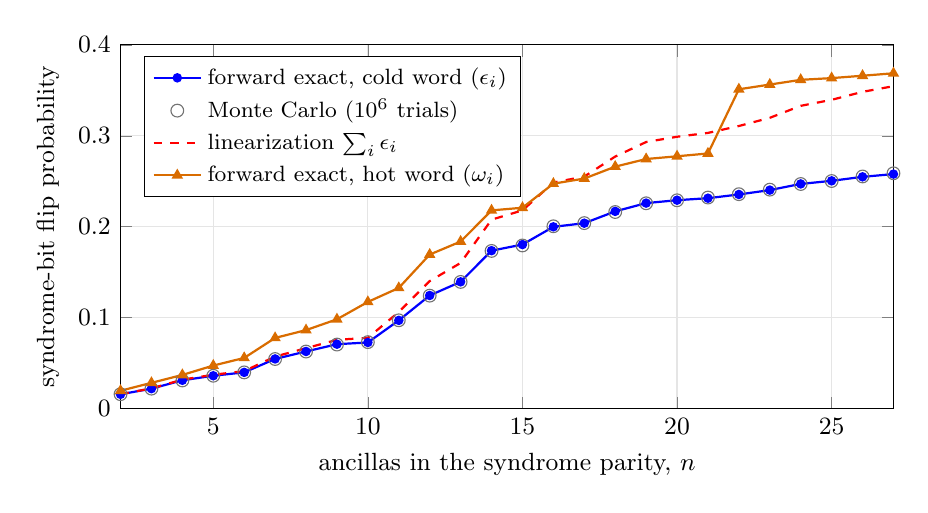
\begin{tikzpicture}
\begin{axis}[
  width=0.94\linewidth, height=6.2cm,
  xlabel={ancillas in the syndrome parity, $n$},
  ylabel={syndrome-bit flip probability},
  xmin=2, xmax=27, ymin=0, ymax=0.4,
  legend pos=north west, legend cell align=left,
  grid=major, grid style={gray!20}, tick label style={font=\small},
  label style={font=\small}, legend style={font=\footnotesize},
]
\addplot[blue, thick, mark=*, mark size=1.3pt] coordinates {
(2,0.0157) (3,0.0219) (4,0.0311) (5,0.0361) (6,0.0398) (7,0.0546) (8,0.0628) (9,0.0708) (10,0.0727) (11,0.0970) (12,0.1244) (13,0.1394) (14,0.1737) (15,0.1804) (16,0.1999) (17,0.2039) (18,0.2169) (19,0.2260) (20,0.2292) (21,0.2314) (22,0.2355) (23,0.2403) (24,0.2471) (25,0.2505) (26,0.2549) (27,0.2579) };
\addlegendentry{forward exact, cold word ($\eps_i$)}
\addplot[only marks, mark=o, mark size=2.3pt, black!55] coordinates {
(2,0.0158) (3,0.0219) (4,0.0309) (5,0.0361) (6,0.0398) (7,0.0545) (8,0.0627) (9,0.0704) (10,0.0731) (11,0.0971) (12,0.1242) (13,0.1393) (14,0.1734) (15,0.1794) (16,0.2005) (17,0.2040) (18,0.2162) (19,0.2258) (20,0.2291) (21,0.2321) (22,0.2358) (23,0.2408) (24,0.2470) (25,0.2503) (26,0.2553) (27,0.2588) };
\addlegendentry{Monte Carlo ($10^6$ trials)}
\addplot[red, thick, dashed] coordinates {
(2,0.0158) (3,0.0222) (4,0.0318) (5,0.0372) (6,0.0412) (7,0.0572) (8,0.0664) (9,0.0756) (10,0.0778) (11,0.1062) (12,0.1402) (13,0.1602) (14,0.2078) (15,0.2180) (16,0.2486) (17,0.2552) (18,0.2772) (19,0.2932) (20,0.2990) (21,0.3032) (22,0.3108) (23,0.3198) (24,0.3330) (25,0.3396) (26,0.3484) (27,0.3546) };
\addlegendentry{linearization $\sum_i \eps_i$}
\addplot[orange!85!black, thick, mark=triangle*, mark size=1.6pt] coordinates {
(2,0.0196) (3,0.0283) (4,0.0370) (5,0.0473) (6,0.0557) (7,0.0777) (8,0.0863) (9,0.0982) (10,0.1173) (11,0.1327) (12,0.1694) (13,0.1837) (14,0.2180) (15,0.2209) (16,0.2474) (17,0.2530) (18,0.2661) (19,0.2745) (20,0.2775) (21,0.2806) (22,0.3512) (23,0.3564) (24,0.3616) (25,0.3635) (26,0.3661) (27,0.3688) };
\addlegendentry{forward exact, hot word ($\omega_i$)}
\end{axis}
\end{tikzpicture}
\caption{The forward calculus on the real readout calibration of
\texttt{ibm\_hanoi} ($27$ qubits, $2025$-$02$-$26$). For a syndrome parity of the
first $n$ qubits, the closed form~\eqref{eq:parity-asym} (solid) coincides with a
$10^6$-shot Monte Carlo of the same channels (circles) to within $10^{-3}$
throughout, confirming the formula on real rates. The linearization
$\sum_i \eps_i$ (dashed) overestimates the cold-word error, by $37\%$ at $n=27$,
and keeps climbing while the exact value saturates toward $\tfrac12$; it is the
\emph{cold} parity's linearization, and the hot parity's own linearization
$\sum_i \omega_i$ (not drawn) lies above the hot curve. The gap
between the cold curve ($\eps_i$, every ancilla truly in $\ket{0}$) and the hot
curve ($\omega_i$, every ancilla in $\ket{1}$), about $0.11$ at $n=27$, is the
readout asymmetry that a single symmetrized rate cannot represent. Reproduced by
\texttt{code/readout\_figure.py}, which carries the calibration snapshot inline.}
\label{fig:realcalib}
\end{figure}

Three things are visible at once on real calibration numbers. The closed form sits exactly
on the simulated points, so the calculus is not a bound but the exact error of the
model on real rates. The linearization runs above the truth and keeps climbing
past $\tfrac12$, the regime \cref{sec:worked} flagged as unphysical. And the cold
and hot curves separate by more than a tenth at the largest parities, the $T_1$
asymmetry that a one-rate model averages away and that \cref{cor:parity-asym}
keeps.

\begin{remark}[Majority vote and feed-forward, in one line each]
A \emph{majority} of $2m+1$ independent measured copies of one latent bit has
error $\sum_{k=m+1}^{2m+1}\binom{2m+1}{k} r^k (1-r)^{2m+1-k}$ on the conditioned
side with flip rate $r\in\{\eps,\omega\}$, the Bernoulli amplification rule,
which (unlike coherent amplitude amplification) requires a stable resampleable
latent value, here repeated readout of a fixed computational-basis value.
A \emph{feed-forward conditional} ``apply $G$ if $b=1$'' fires erroneously with
probability $\eps$ when it should not and is skipped erroneously with probability
$\omega$ when it should fire; down a chain of conditionals,
\cref{cor:composition} gives the probability that \emph{some} stage errs, which
bounds but need not equal the final-output error when errors can cancel; the
latter needs \cref{prop:tensor} at the relevant latent word.
\end{remark}

\subsection{Crosstalk sensitivity, quantified}
\label{sec:worked-crosstalk}

How wrong is the independent prediction when the channels are correlated, and
how much of the gap does the first-order rate of \cref{prop:corrparity}
recover? \Cref{tab:crosstalk} answers on the same real rates (the first $8$
qubits of the \texttt{ibm\_hanoi} calibration), for two dependence structures
chosen to bracket the answer, each with an exact ground truth computed by
conditioning on the crosstalk events.

\paragraph{Chain crosstalk (pairwise-dominated).} A shared flip-cause
$C_e\sim\mathrm{Bern}(\lambda)$ on each adjacent pair $e=(i,i+1)$, OR'd into
both endpoints, models readout crosstalk between neighboring resonators:
adjacent covariances are $O(\lambda)$ while all higher central cross-moments
are $O(\lambda^2)$. Two things happen at once in \cref{tab:crosstalk}. First,
the parity is nearly immune to this crosstalk: the correlated flips arrive in
adjacent \emph{pairs} and cancel in the parity, so the exact error barely moves
from its crosstalk-free value of $\approx0.063$. Second, the \emph{independent}
prediction, computed from the model's own (crosstalk-inflated) marginal rates,
overestimates badly, by a factor of $2.8$ at $\lambda=0.01$ and $5.8$ at
$\lambda=0.05$. This is exactly the situation of a practitioner who calibrates
per-qubit marginal rates on hardware (marginals silently absorb crosstalk) and
then assumes independence. The first-order rate recovers the bulk of the gap,
with the $O(\lambda^2)$ residual visible in the table.

\paragraph{Global common cause (all-order).} One event OR'd into every bit
puts \emph{every} central cross-moment at $\Theta(\lambda)$, each order $|T|$
entering at first order in $\lambda$, the structure a pairwise truncation
cannot see.
The first-order rate fails immediately, even leaving $[0,1]$, while the full
expansion of \cref{eq:corrparity}, all terms kept, equals the
directly-conditioned truth by construction. The contrast is the point: the
validity of the first-order correction is a property of the dependence
\emph{structure}, pairwise-dominated or not, and not merely of the correlation
strength. At extreme coupling the dependence can even overturn the first-order
sign: on nine qubits at $\lambda=\tfrac12$ the global model's exact error
($0.535$) sits \emph{above} its independent anchor ($0.500$), the reversal
\cref{cor:crosstalk-sign} warns of.

\paragraph{Comparison with an established cumulant reconstruction.} The
first-order rate~\eqref{eq:corrparity-fo} keeps at most one covariance factor
per term. \citet{hamilton2020scalable} reconstruct multi-qubit readout
distributions from one- and two-qubit conditional cumulants. Projected onto
parity, with all pair covariances kept in every partial matching and cumulants
of order above two set to zero, that construction is a stronger baseline than
the truncation here. On the chain model at $\lambda=0.01$ it gives $0.0643$
against the exact $0.0623$, where the first-order rate gives $0.0735$; at
$\lambda=0.05$ it gives $0.110$ against the exact $0.070$, where the
first-order rate gives $0.228$. (These baseline values were computed for the
October 2026 revision of this preprint; they are not reported by Hamilton et
al.) The pairwise correction of \cref{prop:corrparity} is therefore weaker
than the established reconstruction, and neither removes the need for
higher-order information under a global common cause.

\begin{table}[t]
\centering
\caption{Correlated-parity validation on the first $8$ qubits of the
\texttt{ibm\_hanoi} calibration. For each crosstalk-event rate $\lambda$: the
prediction assuming independence at the model's own marginals, the first-order
rate~\eqref{eq:corrparity-fo}, and the exact error by conditioning on the
crosstalk events (a $2\times10^6$-trial Monte Carlo agrees to within
$10^{-3}$). Chain crosstalk: adjacent flips cancel in the parity, the
independent prediction overestimates up to $5.8\times$, and the first-order
rate tracks the truth with $O(\lambda^2)$ error. Global common cause: every
cumulant order is $O(\lambda)$ and the first-order rate fails, even leaving
$[0,1]$. Reproduced by \texttt{code/crosstalk\_validation.py}.}
\label{tab:crosstalk}
\small
\begin{tabular}{c rrr @{\hskip 2em} rrr}
\toprule
 & \multicolumn{3}{c}{chain crosstalk} & \multicolumn{3}{c}{global common cause} \\
\cmidrule(r{2em}){2-4} \cmidrule{5-7}
$\lambda$ & indep. & first order & exact & indep. & first order & exact \\
\midrule
0.001 & 0.0749 & 0.0628 & 0.0626 & 0.0698 & \phantom{$-$}0.0206 & 0.0627 \\
0.005 & 0.1207 & 0.0654 & 0.0624 & 0.0968 & $-$0.1364 & 0.0624 \\
0.010 & 0.1717 & 0.0735 & 0.0623 & 0.1285 & $-$0.3078 & 0.0621 \\
0.020 & 0.2556 & 0.1019 & 0.0628 & 0.1855 & $-$0.5770 & 0.0615 \\
0.050 & 0.4050 & 0.2283 & 0.0703 & 0.3132 & $-$0.9370 & 0.0596 \\
\bottomrule
\end{tabular}
\end{table}


\section{Related work and positioning}
\label{sec:related}

We situate the calculus against five neighbors, citing each and stating the
distinction; the claimed-versus-not-claimed boundary itself is collected once,
in \cref{sec:scope}.

\paragraph{(a) Matrix-inversion readout mitigation (the inverse paradigm).}
M3 \citep{nation2021m3}, the multiqubit treatment of
\citet{bravyi2021mitigating}, and tensored/local assignment-matrix mitigators
build the assignment matrix $A$ (our~\eqref{eq:kron}) and approximately invert it
to recover an ideal distribution from observed counts. This is an \emph{inverse},
\emph{numerical}, \emph{per-circuit} procedure operating on measured data. The
work nearest our motivating examples is the mid-circuit-measurement and
feed-forward readout mitigation of \citet{koh2024readout}, which targets exactly
the derived and fed-forward readouts we post-process; it too is an inverse
mitigation of measured outcomes, not a forward symbolic rate calculation. The
forward calculation here is its complement: given the rates, predict and budget
the error on a specific derived bit, symbolically, before data. General
asymmetric response matrices, and tensor products of asymmetric single-qubit
matrices, are already standard in this literature; \citet{smith2021bitflip}
work with them explicitly before symmetrizing the channel on purpose by
physical bit-flip averaging. On the design-time side,
detector-error-model tooling \citep{gidney2021stim} composes per-mechanism flip
probabilities through parities exactly, but numerically, per circuit, and
symmetrically; the closed forms here are a symbolic, asymmetric counterpart.
The tensored assignment
matrix is the linear-algebra shadow of our \cref{prop:tensor}; we add the
symbolic forward layer over it and never invert anything. The two are
complementary, not competing, one designs the budget, the other cleans the
data.

\paragraph{(b) Effectus theory / Adams--Jacobs type theory.}
Effectus theory and the Adams--Jacobs type theory for probabilistic and Bayesian
reasoning \citep{cho2015effectus,adams2015typetheory} give a categorical
``algebra of predicates'' in which predicates form effect algebras and Boolean
and probabilistic logic appear as special cases of the quantum case, the same
structural DNA as a typed calculus of predicates under noise. It is, however, a
\emph{foundation for the structure} of probabilistic and quantum theory and for
Bayesian conditioning; it is not a device readout-error model and carries no
$(\eps,\omega)$ rate-propagation rules. The distinction is \emph{rates}: the
present paper propagates numbers, not just predicate structure. The closer
predecessor for rate propagation is the circuit-reliability literature
in~(c).

\paragraph{(c) Parity identities and forward error propagation in logic
circuits.} The parity formula~\eqref{eq:parity} is Lemma~1 of
\citet{gallager1962ldpc} and the piling-up lemma of \citet{matsui1993linear};
the exact $\pm1$/Fourier parity-bias identity is standard in the analysis of
Boolean functions \citep{odonnell2014}, and the reliability of noisy Boolean
formulas is the tradition of \citet{vonneumann1956} and \citet{pippenger1988}.
Forward propagation of error through combinational networks with asymmetric,
input-dependent probabilities is also established: \citet{parker1975probabilistic}
compute signal probabilities through general combinational networks, and
probabilistic transfer matrices \citep{krishnaswamy2008ptm} treat
input-pattern-dependent errors, error probabilities for individual input words,
averaging over joint input distributions, and reconvergent fan-out, with serial
and tensor composition. Applying those operations to imperfect input wires
followed by ideal gates reproduces \cref{sec:calculus}. The latent-conditioned
two-rate bookkeeping (\cref{prop:not,thm:andor,cor:parity-asym,prop:tensor}) is
therefore a specialization of known methods to readout, not a new calculus.

\paragraph{(d) Asymmetric quantum hypothesis testing / channel certification.}
A two-sided false-positive/false-negative model of a \emph{single} measurement
already appears in asymmetric quantum hypothesis testing and channel
certification, for instance the false-negative-free certification of
\citet{krawiec2021certification}. This is the nearest neighbor of our atom
(\cref{def:atom}) and we cite it to preempt ``this is just type~I/II error.'' The
difference is the \emph{composition layer}: those works study one decision,
while this paper composes \emph{many} measured bits through Boolean
combinations and tensoring, using the established methods of~(c).

\paragraph{(e) Asymmetry-from-relaxation physics.}
\citet{tannu2019mitigating} establish and exploit state-dependent (asymmetric)
readout bias from $T_1$ relaxation, with measured errors of roughly $8$--$30\%$;
\citet{hicks2021readout} use the same asymmetry via readout rebalancing. These
motivate \cref{def:atom} and \cref{rem:t1}, they are the source of the $\omega>\eps$
regime our calculus is built to preserve. They mitigate; we propagate.

\paragraph{Unification with classical probabilistic data structures.}
Finally, the setting is the error model of Bernoulli
type theory, the framework of random approximate sets, maps, and relations whose
special cases include Bloom filters \citep{bloom1970}, perfect hash filters, and
cipher maps \citep{bernoulliSets,bernoulliComposition,bernoulliMaps,bernoulliRelations}.
For self-containedness the unification needs no external reference: a random
approximate set is the membership indicator of a set $A$, reported through an
independent per-element asymmetric channel~\eqref{eq:channel} with false-positive
rate $\eps$ on nonmembers and false-negative rate $\omega$ on members, and set
operations compose those rates by the closed forms of \cref{sec:calculus},
conditioned on each element's membership pattern in the operands (so the
composed set generally has a higher model order than two
\citep{bernoulliComposition}). The
companion papers develop the consequences, but the unification claim rests only on
this one-line model.
A Bloom filter is the one-sided ($\omega=0$) corner; a $T_1$-biased syndrome
ancilla is an asymmetric interior point; both obey the same
\cref{prop:not,thm:andor,thm:parity,cor:composition}. Recognizing quantum readout
as an instance of this model is what lets a single calculus serve a classical
data structure and a quantum-hardware error budget at once.


\section{Scope and limitations}
\label{sec:scope}

We state the boundaries plainly, to forestall overclaiming.

\begin{enumerate}[leftmargin=1.6em]
  \item \textbf{Forward, not inverse.} The contribution predicts and budgets the
        error of a derived bit from given per-qubit rates. It does \emph{not}
        recover an ideal distribution from observed counts and is \emph{not} a
        competitor to M3 or other mitigation; it is their design-time complement
        \citep{nation2021m3,bravyi2021mitigating}.

  \item \textbf{Independence is assumed, and is the reference point.} Every closed
        form above holds under per-bit channel independence, equivalently, the
        tensored assignment matrix~\eqref{eq:kron}. Real devices exhibit
        \emph{measurement crosstalk}: the readout of one qubit is correlated with
        the state or readout of its neighbors, which is why correlated models such
        as the continuous-time Markov process (CTMP) model of
        \citet{bravyi2021mitigating} exist. Independence can also fail
        \emph{structurally} rather than physically: a single readout reused across
        several inputs of the derived bit (reconvergent fan-out, \cref{sec:calculus})
        correlates those inputs exactly as crosstalk does, so a derived bit that is
        not a fan-out-free tree needs the same non-factorized treatment. The
        independent prediction is best read
        as the correlation-free \emph{reference}: it is exact given the per-qubit
        marginals alone, and the leading correction is now quantified rather
        than merely signed. \Cref{prop:corrparity} expands a parity's error
        exactly in the dependence structure; \cref{cor:crosstalk-sign} reads
        off the first-order sign (positively correlated misreads make
        coincident flips more likely and push the parity error \emph{below}
        the independent value, negatively correlated ones push it \emph{above},
        to first order); and \cref{sec:worked-crosstalk} shows the first-order
        rate tracking the exact one under pairwise-dominated (neighbor-chain)
        crosstalk while failing, honestly and visibly, under a global common
        cause whose higher cumulants enter at the same order. The independent
        rate is thus a first-order anchor, not a worst case. Bounding the
        remainder for a given CTMP generator, and a non-factorized lift of the
        remaining Boolean operations, stay future work; the present calculus is
        exact in the independent/tensor regime and first-order beyond it.

  \item \textbf{Fixed-basis readout statistics only.} The latent-value model is
        exact for the outcome statistics of one fixed-basis measurement, for any
        input state, whenever the detector's effects are diagonal in that basis
        (\cref{eq:povm}); coherent and entangled inputs are not excluded. It
        does not provide a single joint distribution across incompatible
        measurement settings (the content of the Bell / Kochen--Specker / Fine
        obstructions, outside our scope here), and it says nothing about
        pre-measurement coherences or amplitude amplification, which do not
        enter~\eqref{eq:povm}. Detectors whose effects are not diagonal in the
        measurement basis fall outside the model. Our claims concern the bits a
        device reports in one basis.

  \item \textbf{Originality, precisely.} Not claimed: the single-bit asymmetric
        channel (\cref{def:atom}); the tensor factorization of independent-qubit
        readout (\cref{eq:kron}) and asymmetric response matrices
        \citep{smith2021bitflip}; the parity formula~\eqref{eq:parity}
        \citep{gallager1962ldpc,matsui1993linear}; forward propagation of
        input-dependent error through Boolean networks, of which
        \cref{sec:calculus} is a specialization
        \citep{parker1975probabilistic,krishnaswamy2008ptm}; and the pairwise
        crosstalk truncation as a method, which is weaker than the cumulant
        reconstruction of \citet{hamilton2020scalable}. A single
        $(\eps,\omega)$ pair does not propagate through a general tree
        (\cref{rem:no-pair}); rates are carried per latent assignment. What
        the paper offers: these known tools applied to readout-derived bits;
        worked numbers on the \texttt{ibm\_hanoi} calibration (the linear rule
        overestimates the $27$-qubit cold-word parity error by $37\%$); and the
        identification of readout error with the Bernoulli error model of
        classical probabilistic data structures.

  \item \textbf{Empirical validation.} This is a methods/perspective paper.
        \Cref{sec:worked-real} checks the closed forms against a direct Monte Carlo
        simulation on the published readout calibration of a real device,
        confirming them on hardware-realistic rates. What remains open is a
        \emph{live-hardware} study comparing predicted derived-bit rates against
        \emph{measured} ones, and quantifying the independence-violation gap from
        crosstalk; that would strengthen the claims further but is beyond this
        draft. We make no empirical claim beyond the exactness of the derivations
        under the stated independence assumption and the simulation check of
        \cref{sec:worked-real}.
\end{enumerate}


\section{Conclusion}
\label{sec:conclusion}

For a detector with diagonal measurement effects, quantum readout error is a
classical asymmetric bit-flip channel on the fixed-basis statistics of any
state, and the bits a quantum program reports are Boolean functions of such
channels. We have applied the known forward calculation, evaluated per latent
assignment, that gives the error of a derived bit from the per-qubit rates
$(\eps_i,\omega_i)$ through negation, conjunction, disjunction, parity, chains,
and independent-qubit tensoring. The rates are carried per latent word; a
single $(\eps,\omega)$ pair does not survive general composition
(\cref{rem:no-pair}). The lead example, the reliability of a syndrome bit, is
$\tfrac12\bigl(1-\prod_i(1-2r_i)\bigr)$, Gallager's parity identity with
latent-conditioned flip rates, which the folklore ``$n$ times the
per-measurement error'' rule overestimates by tens of percent at modest sizes
and rates.

The calculation is deliberately bounded: forward rather than inverse,
complementary to matrix-inversion mitigation; exact under per-bit independence
and first-order beyond it (\cref{sec:crosstalk}), where an established cumulant
reconstruction does better; and restricted to fixed-basis readout statistics.
The same object that governs Bloom filters and cipher maps budgets the error of
a quantum-measurement post-processing pipeline without forming the exponential
assignment matrix. The natural next steps are a
beyond-first-order correlated-channel (CTMP-regime) lift of the same
operations, seeded by the exact dependence expansion of \cref{prop:corrparity},
and a \emph{live-hardware} study of predicted against measured derived-bit
rates, beyond the simulation validation of
\cref{sec:worked-real,sec:worked-crosstalk}.

\paragraph{Acknowledgments.} This work is part of the Bernoulli type theory
program; the readout connection was developed in a concept note dated 2026-06-06.

\bibliography{references}

\end{document}
